\chapter{System Analysis}
\begin{spacing}{1}
\setlength{\parskip}{0.3in}
\graphicspath{{./Chapter3/}}

\section{Information Gathering}
Information Gathering is a very key part of the feasibility analysis process. Information gathering is both an art and a science. It is a science because it requires a proper methodology and tools in order to be effective. It is an art too, because it requires a sort of mental dexterity to achieve the best results.

\subsection{Information Gathering Tools}
For gathering information we have to go through many processes.Mainly we collect our data from:
\begin{enumerate}
\item Online Survey
\item Akash DTH FAQ section 
\end{enumerate}
And finally we are lucky to manage a meeting with a manager of akash DTH,we asked him many questions and found our required data.

\subsection{Questionnaires Analysis}
Following questions were asked in online survey to the customers 

{\bf 1.} Why do you prefer Akash DTH over cable?\newline
{\bf Tables \& Graph}
\begin{figure}[H]
	\centering
	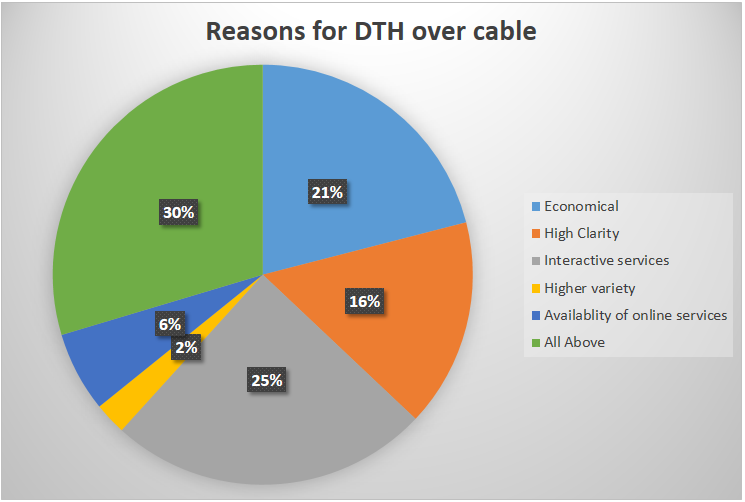
\includegraphics[width=0.8\textwidth]{fig1}
	\caption{Pie Chart showing selecting reasons of DTH}
	\label{fig:PieChart1}
\end{figure}
{\bf Conclusion:}\newline
Most of the Customers prefer Akash DTH over cable because of economical friendly and High quality performance which is far better than cable.

{\bf 2.} How much do you pay for your Akash DTH connection per month?\newline
{\bf Tables \& Graph}\newline
\begin{figure}[H]
	\centering
	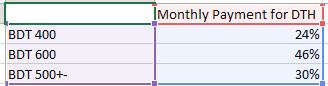
\includegraphics[width=0.8\textwidth]{fig2_1}
	\caption{users monthly payments}
	\label{fig:Table1}
\end{figure}
\begin{figure}[H]
	\centering
	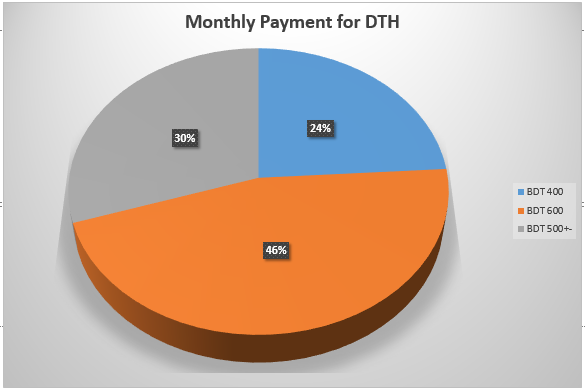
\includegraphics[width=0.8\textwidth]{fig2_2}
	\caption{Pie Chart showing users monthly payment}
	\label{fig:pieChar2}
\end{figure}
{\bf Conclusion: }\newline
Most the customer of Akash DTH purchases 400 BTD/month package

{\bf 3.} How would you rate your satisfaction from yours DTH provider?\newline
{\bf Tables \& Graph}\newline
\begin{figure}[H]
	\centering
	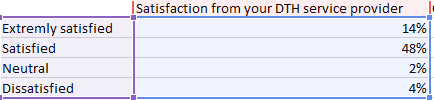
\includegraphics[width=0.8\textwidth]{fig3_2}
	\caption{user satisfaction}
	\label{fig:Table2}
\end{figure}
\begin{figure}[H]
	\centering
	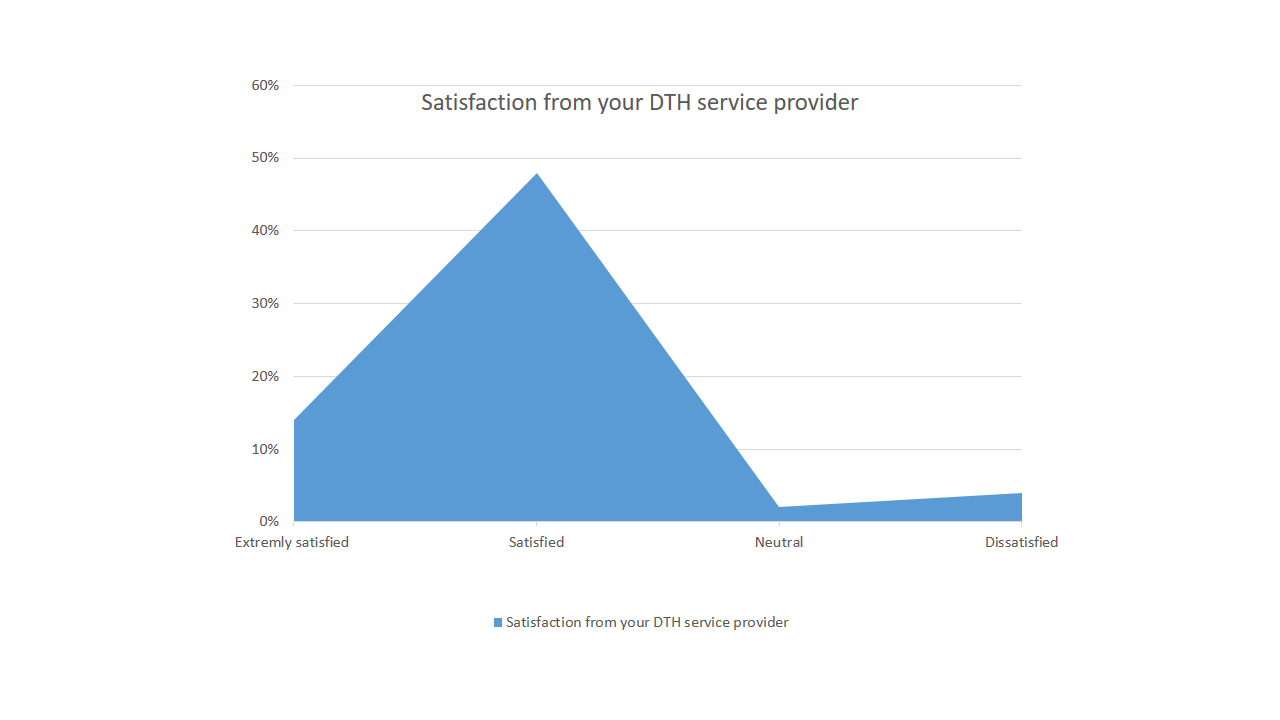
\includegraphics[width=1.2\textwidth]{fig3_1}
	\caption{Graph showing user satisfaction percentage}
	\label{fig:g1}
\end{figure}
{\bf Conclusion: }\newline
Maximum number of customers are satisfied with akash DTH provider.

{\bf 4.} How many channels do you get in your akash DTH package?\newline
{\bf Tables \& Graph}\newline
\begin{figure}[H]
	\centering
	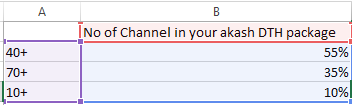
\includegraphics[width=0.8\textwidth]{fig4_1}
	\caption{number of channels in packages}
	\label{fig:Table3}
\end{figure}
\begin{figure}[H]
	\centering
	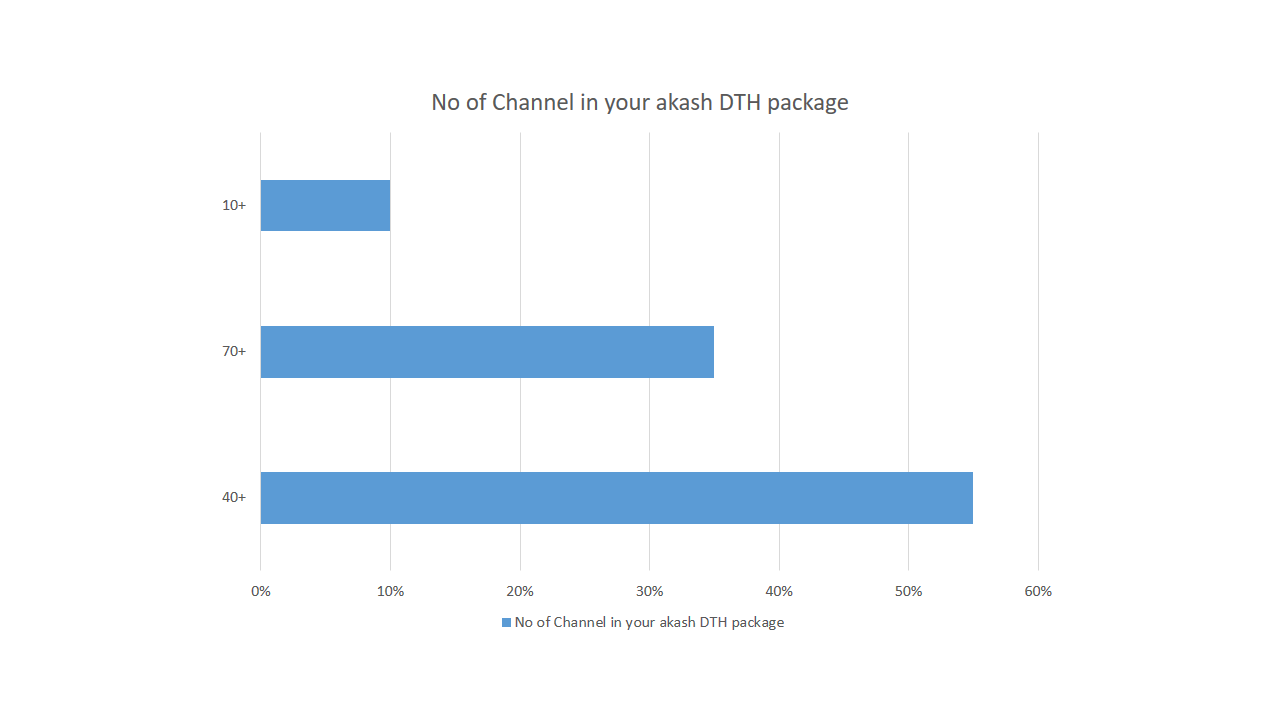
\includegraphics[width=1.2\textwidth]{fig4_2}
	\caption{Bar Chart showing numbers of channels in packages}
	\label{fig:bar1}
\end{figure}
{\bf Conclusion: }\newline
Akash Basic Package serves 40+ channel which is standard for most of the customers.

{\bf 5.} Do you easily get recharge your akash DTH?\newline
{\bf Tables \& Graph}\newline
\begin{figure}[H]
	\centering
	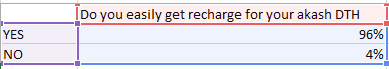
\includegraphics[width=0.8\textwidth]{fig5_1}
	\caption{percentage of users with ease of recharge}
	\label{fig:Table4}
\end{figure}
\begin{figure}[H]
	\centering
	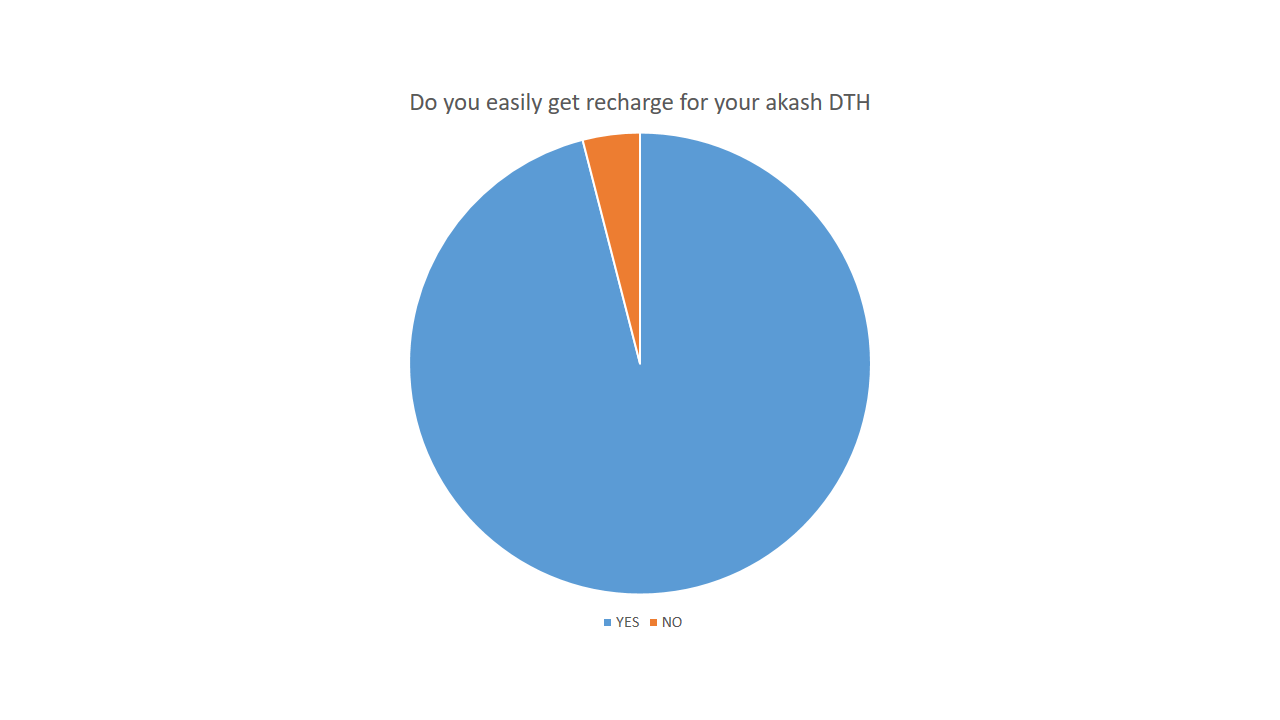
\includegraphics[width=0.8\textwidth]{fig5_2}
	\caption{Pie chart showing percentage of users with ease of recharge}
	\label{fig:pie3}
\end{figure}
{\bf Conclusion: }\newline
Akash DTH provide every types of payment access in Bangladesh.example : Bkash,Rocket,DBBL,Nagad,Bank Payment,Card Payment etc.So it is too much easy for most of the customer.

\section{Overview of Existing System}
\begin{figure}[H]
	\centering
	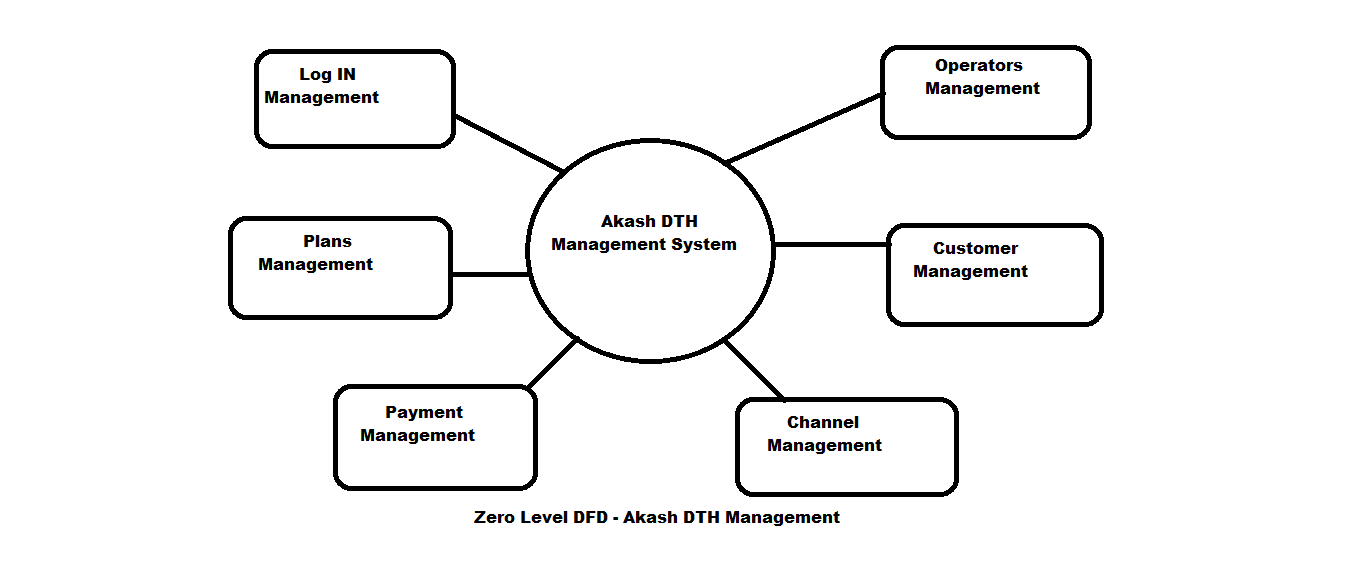
\includegraphics[width=1.2\textwidth]{DFD1}
	\caption{Akash DTH Management - Zero Level DFD}
	\label{fig:dfd1}
\end{figure}
\begin{figure}[H]
	\centering
	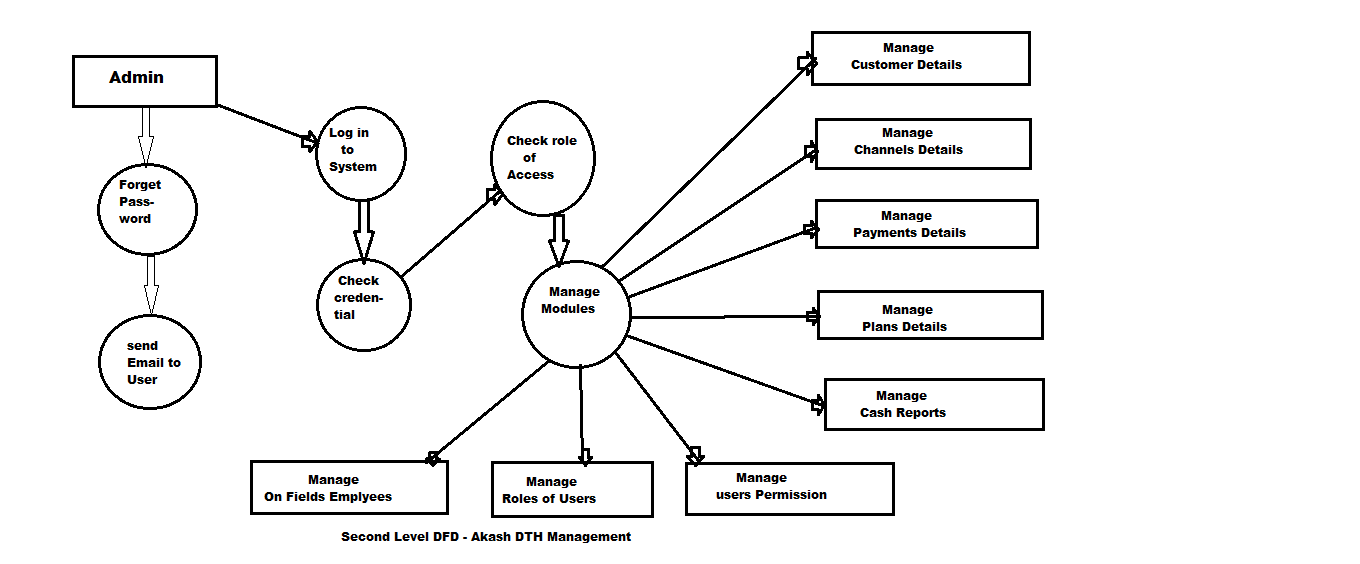
\includegraphics[width=1.2\textwidth]{DFD2}
	\caption{Akash DTH Management - Second Level DFD}
	\label{fig:dfd2}
\end{figure}
\subsection{Description of DFDs}
DFD is a most important Diagram for any System Management.Akash DTH maintains a well structured DFD Diagram for their management.Initially Akash DTH divided their management into several sub management module.The Head management managers control the sub management modules.In each sub-management module there is a group of people to manage field level employees.

\subsection{Customer Management Module}
customer management module is responsible for any types of customers complains,they generally collect data from customer phone call or physical investigation,generally they propose the upcoming customers requirements and plans.All other sub-modules works in the same flow. 

\subsection{Channel Management Module}
Channel Management Module is a vital management module.They have to conscious about customer requirements,which types of channels are mostly liked by customer. They have to Organize channels package which will satisfy customer requirements.

\subsection{Log In Management Module}
Log in management module is a small part of Akash DTH management module.A small group of tech-employee manage the Authorization of access in Akash DTH server.

\subsection{Payment Management Module}
Payment management module is the second most vital management module.They have to ensure that every customer pays their monthly bill,if any customer didn't pay his bill then they are responsible for convince the customer to pay the bill as early as possible or the will disconnect their service, and they also collaborate with different various bill payment companies to manage akash bill payment most easily.

\subsection{Plans Management Module}
Plans Management Teams discover various types of package to attract customers. 

\section{Feasibility Analysis}
The process of describing, identifying, and evaluating the proposed system, as well as selecting the optimal system for proper operation, is referred to as feasibility. A feasibility study is carried out in order to determine whether the system can be developed or not. A feasibility study might be one of three sorts.
They are : 
\begin{itemize}
\item  Technical feasibility 
\item  Economical feasibility 
\item  Behavioral feasibility
\end{itemize}
\subsection{Technical feasibility}
Technical feasibility aids in gaining access to present resources as well as technology needed to meet the user's requirements in the system within the budget and schedule constraints. In the technical feasibility, the following tasks are completed:
Assists in determining the stability of the technology in use.
The technological system of Akash DTH should be upgraded.A customer management feature should be included.
\subsection{ Economical feasibility }
 Economic Feasibility helps in determining whether the required system has the potential to generate financial gains for an organization.System can be considered to be feasible only if it focuses on the issues that are discussed below:
\begin{itemize}
\item  The cost associated with the customer service team ,training, development team, software and hardware.
\item  Cost required for conducting system investigation such as requirements analysis and requirements elicitation.
\item  The cost incurred on the development of a system for producing long-term gains for an organization.
\end{itemize}
The current Akash DTH technology is quite cost-effective. However, in order to achieve more economic growth, the system must be improved.

\subsection{Behavioral feasibility}
The study of behavioral feasibility is done to see if humans or employees in the firm will use it or not. The following considerations were made during the examination of this suggested system:
Is it simple to use? Is it safe to use?
Is it difficult to operate and maintain?
The current Akash DTH system is not behaviorally feasible.The Customer Management module is difficult to utilize.


\subsection{Feasibility Study}
Main focus of our candidate system is to be a cost effective user friendly system.There are many limitations in the existing system.So that we have found out some of these limitations and proposed a cost effective candidate system.Our candidate system will satisfy our old customer and as well as attract new customer as a result this system will increase revenue of Akash DTH.
The following steps should be taken for the candidate system :-
\subsubsection{Candidate System}
\begin{itemize}
\item {\bf  Customer Management } \newline In order to keep up with the growing number of clients, Akash DTH needs keep a well-organized Customer module. The customer module should be automated, which implies that each customer should be given a customer account through a user-friendly mobile app. All forms of consumer requirements can be reduced with a single user-friendly mobile application.
\item {\bf  Reconsidering the target customers } \newline Up till now, Akash DTH has mostly targeted metropolitan residents seeking improved picture and sound quality. The semi-rural and rural populations should be targeted through Akash DTH. Signals from Akash DTH can be found all around Bangladesh. As a result, those in remote areas where cable networks are unavailable can take use of satellite coverage. In Chittagong hill regions, Shon dip, and Hutia, Akash DTH already has subscribers.As a result, those persons should be their target market.
\item {\bf Backup Earth Station } \newline Currently, Akash DTH operates a single earth station in Gazipur, from which they down-link signals from other satellites and up-link them to their own satellite, ABS 2, from which consumers receive the signal directly through their home dish. The signal in Gazipur is distorted when it rains excessively. They can use that ear if they have another earth station in a less humid location.

\item {\bf  Set Top Box Quality improvising} \newline Akash DTH should change their set-top box (STB) quality. The previous STB had some problems like hitting issues and the others. Which created dissatisfaction among customers. Other DTH operators like Tata Sky, Dish in our neighboring country are offering better quality STB. Some of them are Wi-Fi enabled. So if RealVU can provide a more upgraded STB it will attract more people.
\end{itemize}

\section{Cost and Benefits Analysis }
Cost benefit analysis  it is important to identify cost and benefit factors of a candidate system. Cost-benefit analysis is used to determine the economic feasibility of a system. The total expected costs are weighed against the total expected benefits of a candidate system. If the benefits outweigh the costs over a given period of time, the candidate may be considered to be financially viable.
Cost benefit analysis helps to give management a picture of the costs, benefits and risks. It usually involves comparing alternative investments.
Cost benefit determines the benefits and savings that are expected from the system and compares them with the expected costs.
The cost of a candidate system involves the development cost and maintenance cost. The development costs are one time investment whereas maintenance costs are recurring. The development cost is basically the costs incurred during the various stages of the system development.
\subsection{ Cost and Benefit Categories }
Cost and benefits can be categorized into the following categories.
There are several cost factors. These are ;

\begin{itemize}
\item  Hardware
\item Personnel
\item Facility
\item Operating 
\item Supply costs.
\item Equipment
\item Supplies
\item Overheads
\item Consultants' fees
\end{itemize}

\subsection{Hardware cost}
The biggest cost of Akash DTH is the hardware. A large sum of money is spent on hardware. The cost of satellite maintenance is one of the most significant components of Akash DTH's hardware expenditures. For each consumer, our candidate system recommended a more updated setup box. Aside from the expense of the set-up box and satellite maintenance, Akash DTH is attempting to increase signal coverage throughout Bangladesh, which will necessitate a significant investment in antenna installation.
Hardware expenditures are one of the most significant costs for upgrading devices in our suggested candidate system.
\subsection {Software Cost}
A customer management system based on a mobile application is required by our suggested candidate. For customer management, a well-structured mobile application is essential.
\subsection{Personnel Cost}
It is the money spent on the personnel who worked on the system's development. A large number of retailer points are required for our suggested candidate system, and these retailer points may require more manpower.
\subsection{Operating Cost}
The expenses necessary for the system's day-to-day operation are known as operating costs. The system's upkeep is included in this. This can take the form of maintaining the hardware or application programming, or it can take the form of money given to experts who manage or maintain the system.
\subsection{Supply Cost}
These are variable costs that change in relation to the amount of wire, set up box tools used. These should be estimated and factored into the system's overall cost.

\subsection{ Costs and Benefits Identification}
\subsubsection{Tangible Cost}
The systems analyst and accounting personnel appropriately forecast tangible costs. These are tangible costs in our suggested candidate system.
\begin{itemize}
\item Purchase or Upgrade existing DTH set box for customer 
\item Develop a mobile based customer management Application
\item Set up a new backup station
\end{itemize} 

\subsubsection{Tangible Benefit}
Through the usage of the information system, tangible benefits are gains that can be measured in cash.
These are the projected tangible benefits of our suggested candidate system:

\begin{itemize}
\item Mobile based management applications will reduce a huge amount of employee cost.
\item Our Improved candidate system will attract more new customers.
\item Strong signals will grow customer satisfaction then it will be easy to sell new packages to customers.
\end{itemize}


\subsubsection {Intangible Costs }
Those costs that are difficult to estimate and may not be known.In our proposed candidate system these can be  intangible costs;
\begin{itemize}
\item Application maintenance cost
\item If the automated customer management fails for a certain period of time then it will be difficult to measure the cost.
\end{itemize}

\subsubsection{Intangible Benefits }
Intangible benefits are benefits from use of the information system that are difficult to measure.In our proposed candidate system these are our expected intangible benefits;

\begin{itemize}
\item Customer satisfaction
\item Advance Customer management System
\item Increase new customer 
\item Reduce time consuming tasks
\end{itemize}

\subsubsection {Direct Cost }
Direct costs are those expenses or costs that can be directly associated or contributed with a system.The main component of direct costs are direct material and direct labor used for the manufacturing of a product are direct costs. Benefits of Using Direct Costing Methods:
\begin{itemize}
\item It helps in making a master budget for the year as direct costing provides a variable per unit cost.
\item Once the direct and indirect costs are determined, then it becomes easy for management to identify system expenses.
\item It provides more control to the management on organization operations as direct costing pinpoints the responsibility according to organizational lines.
\end{itemize}
 In our proposed candidate system these are direct costs;
\begin{itemize}
\item Electricity Cost
\item Employees Salary
\item Training Cost
\item Transportation cost
\end{itemize}

\subsubsection{Indirect Cost \& Benefit }
Indirect costs are all expenses that are incurred in the same way for several projects, products, or business activities and cannot be clearly split for particular projects, items, or activities. All costs that could not be classified as direct costs are referred to as indirect costs.Indirect costs, like direct costs, are typically reported in the cost of goods sold, whereas indirect costs are typically recorded in general and administrative expenses.
In our proposed candidate system these are indirect costs;
\begin{itemize}
\item Premises Rent
\item Depreciation of Equipment
\item Utility Expense
\end{itemize}
Indirect benefits are considered as a by-product of System. In our proposed system, these are some indirect benefits;
\begin {itemize}
\item Strong Signal
\item Customer Information
\item Ease of information exchange
\item Storage efficiency and volume
\end{itemize}

\subsubsection{Fixed Cost \& Benefit}
Fixed costs of a system are those costs that will not recur.In our proposed system Improved DTH set box , hardware tools , software construction cost are considered as fixed costs. Selling packages with a DTH setup box are a fixed benefit for our proposed candidate system. 

\subsubsection{Variable Cost \& Benefit}
A variable cost is a corporate expense that changes in proportion to how much a company produces or sells. Variable costs increase or decrease depending on a company's production or sales volume; they rise as production/sell increases and fall as production/sell decreases. In our proposed candidate system, the costs that occur in case of any technical failure are considered as variable costs. 
Table Fixed Costs \& Variable Costs 
\begin{figure}[H]
	\centering
	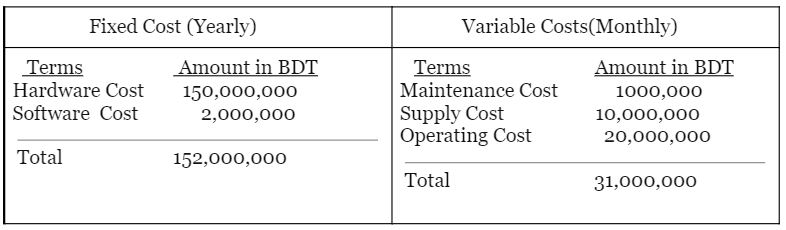
\includegraphics[width=0.8\textwidth]{cost}
	\label{fig:cost}
\end{figure}

\subsection{Evaluation Method of Cost and Benefit }
There are several methods for analyzing costs \& benefits of a system.They are ; 
\begin {itemize}
\item Net Benefit Analysis
\item Present Value Analysis
\item Net Present Value
\item Payback Analysis
\item Break-Even Analysis
\item Cash-Flow Analysis etc
\end{itemize}
For analyzing Akash DTH costs \& benefits here we consider Net benefit analysis and Break-Even Analysis.

\subsubsection{Net Benefit Analysis}
Net Benefit. Net Benefit is determined by summing all benefits and subtracting the sum of all costs of a system. This output provides an absolute measure of benefits.We select this Method because it is easy to measure , interpret \& present.Identifying the yearly cost estimate value of the proposed candidate system of Akash DTH from the previous section.

\[ Total Fixed Cost = 152,000,000 BDT\]
\[Total Variable Cost = 31,000,000 \times 12 = 372,000,000 BDT\]
\[ Total Cost = 524,000,000 BDT\]

Nowadays DTH users are increasing day by day.So we estimated that thousands of new users will use Akash DTH service every month.For our proposed candidate system every year 28\% (estimated) revenue will increase.

Table Net Benefits Analysis:
\begin{figure}[H]
	\centering
	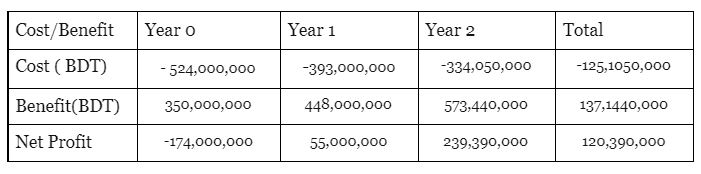
\includegraphics[width=0.8\textwidth]{benefit}
	\label{fig:benefit}
\end{figure}
The main focus of this  candidate system is to satisfy customers, so that we expect that this system will bring financial benefit as well as customer satisfaction.
 
For calculating  the value of the investment after a certain period of  time, the time value of money can be estimated.
The time value of money can be calculated with the following formula,

\begin{equation*}
	\begin{split}
		&\qquad \qquad F = P (1 + i) ^n \\
		&Where, \\
		& F = Future value of an investment  \\
		& P = Present value of an investment \\
		& i =  Interest rate per compounding period \\
		& n =  Number of years Investing 
	\end{split}
\end{equation*}
 524,000,000 BDT for three years at 6 percent interest would have value at maturity of,$ F =  524,000,000 \times (1 + 0.06) ^3  = 624,092,384 BDT $

\subsection{Break Even Analysis}
Break Even Analysis of a system refers to the point in which total cost and total revenue are equal. A break-even point analysis is used to determine the number of units or dollars of revenue needed to cover total costs (fixed and variable costs).Here we used the break-even analysis to compare the cost of the current system \& candidate system.
The current existing Akash DTH system costs 24,000,000 BDT per month as variable cost for maintenance , our proposed 31,000,000 BDT as variable costs for per month initially and fixed cost 152,000,000 BDT yearly.

\subsubsection{Break Even Chart}
\begin{figure}[H]
	\centering
	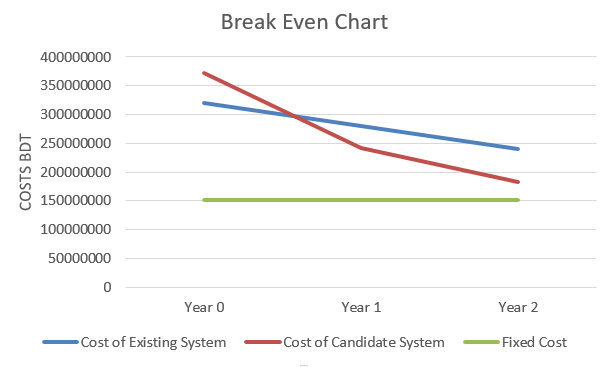
\includegraphics[width=0.8\textwidth]{break}
	\caption {Break Even chart of Akash DTH}
	\label{fig:break}
\end{figure}
From the break-even chart, the break-even point is almost at the year 1 where lines of total cost of existing system and candidate system intersect. At the break-event point, the cost rate of both systems remains the same but the cost rate of the existing system is more after that.


\section{Conclusion}
To analyze and design an information system for any organization, study their working methodology, management system and business policies is the first step. Identifying the problems and limitations of the existing system is the basis for further improvement of 4 that system. In the initial phase, we studied the targeting system of Akash DTH and identified some primary problems with their existing systems.We proposed a candidate system and discussed cost effectiveness and performance of our candidate system against the existing system and verified the economic feasibility, technical feasibility and behavioral feasibility of the candidate system. We analyzed whether our  candidate system can fulfill the organization’s objectives and goals and tried to determine the necessity for the greater development of the organization based on our proposed candidate system. Our candidate system is more feasible and reliable for the organization. Finally, we evaluated cost/benefit analysis for the proposed systems for Akash DTH.
\end{spacing}
